\begin{figure}[H]
\centering
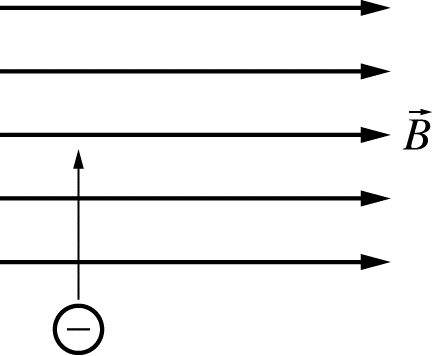
\includegraphics[scale=0.3]{images/img-015-023.png}
\end{figure}

% Multiple Choice Question 34
\begin{questions}\setcounter{question}{33}\question
A negatively charged ion is moving toward the top of the page when it enters a region of space with a uniform magnetic field $\vec{B}$ directed to the right, as shown above. The direction of the force that the magnetic field exerts on the ion is

\begin{choices}
\choice toward the top of the page
\choice to the right
\choice to the left
\choice out of the page
\choice into the page
\end{choices}\end{questions}
